\chapter{Security Practices}\label{ch:security-practices}
Security Practices stuff to talk about:

Security groups limiting HTTP, HTTPS, SSH and MySQL. SSH Connections are limited only to one IP (Eduroam's)

KeyPair for logging into EC2

IAM (But we don't have access)

S3 bucket isn't publicly accessible from the get-go

If we do need public access, it is ONLY for GET or PUT requests (Viewing stories and uploading them)

VPC controlling inbound and outbound traffic

public and private subnets

\begin{figure}[!htbp]
    \centering
    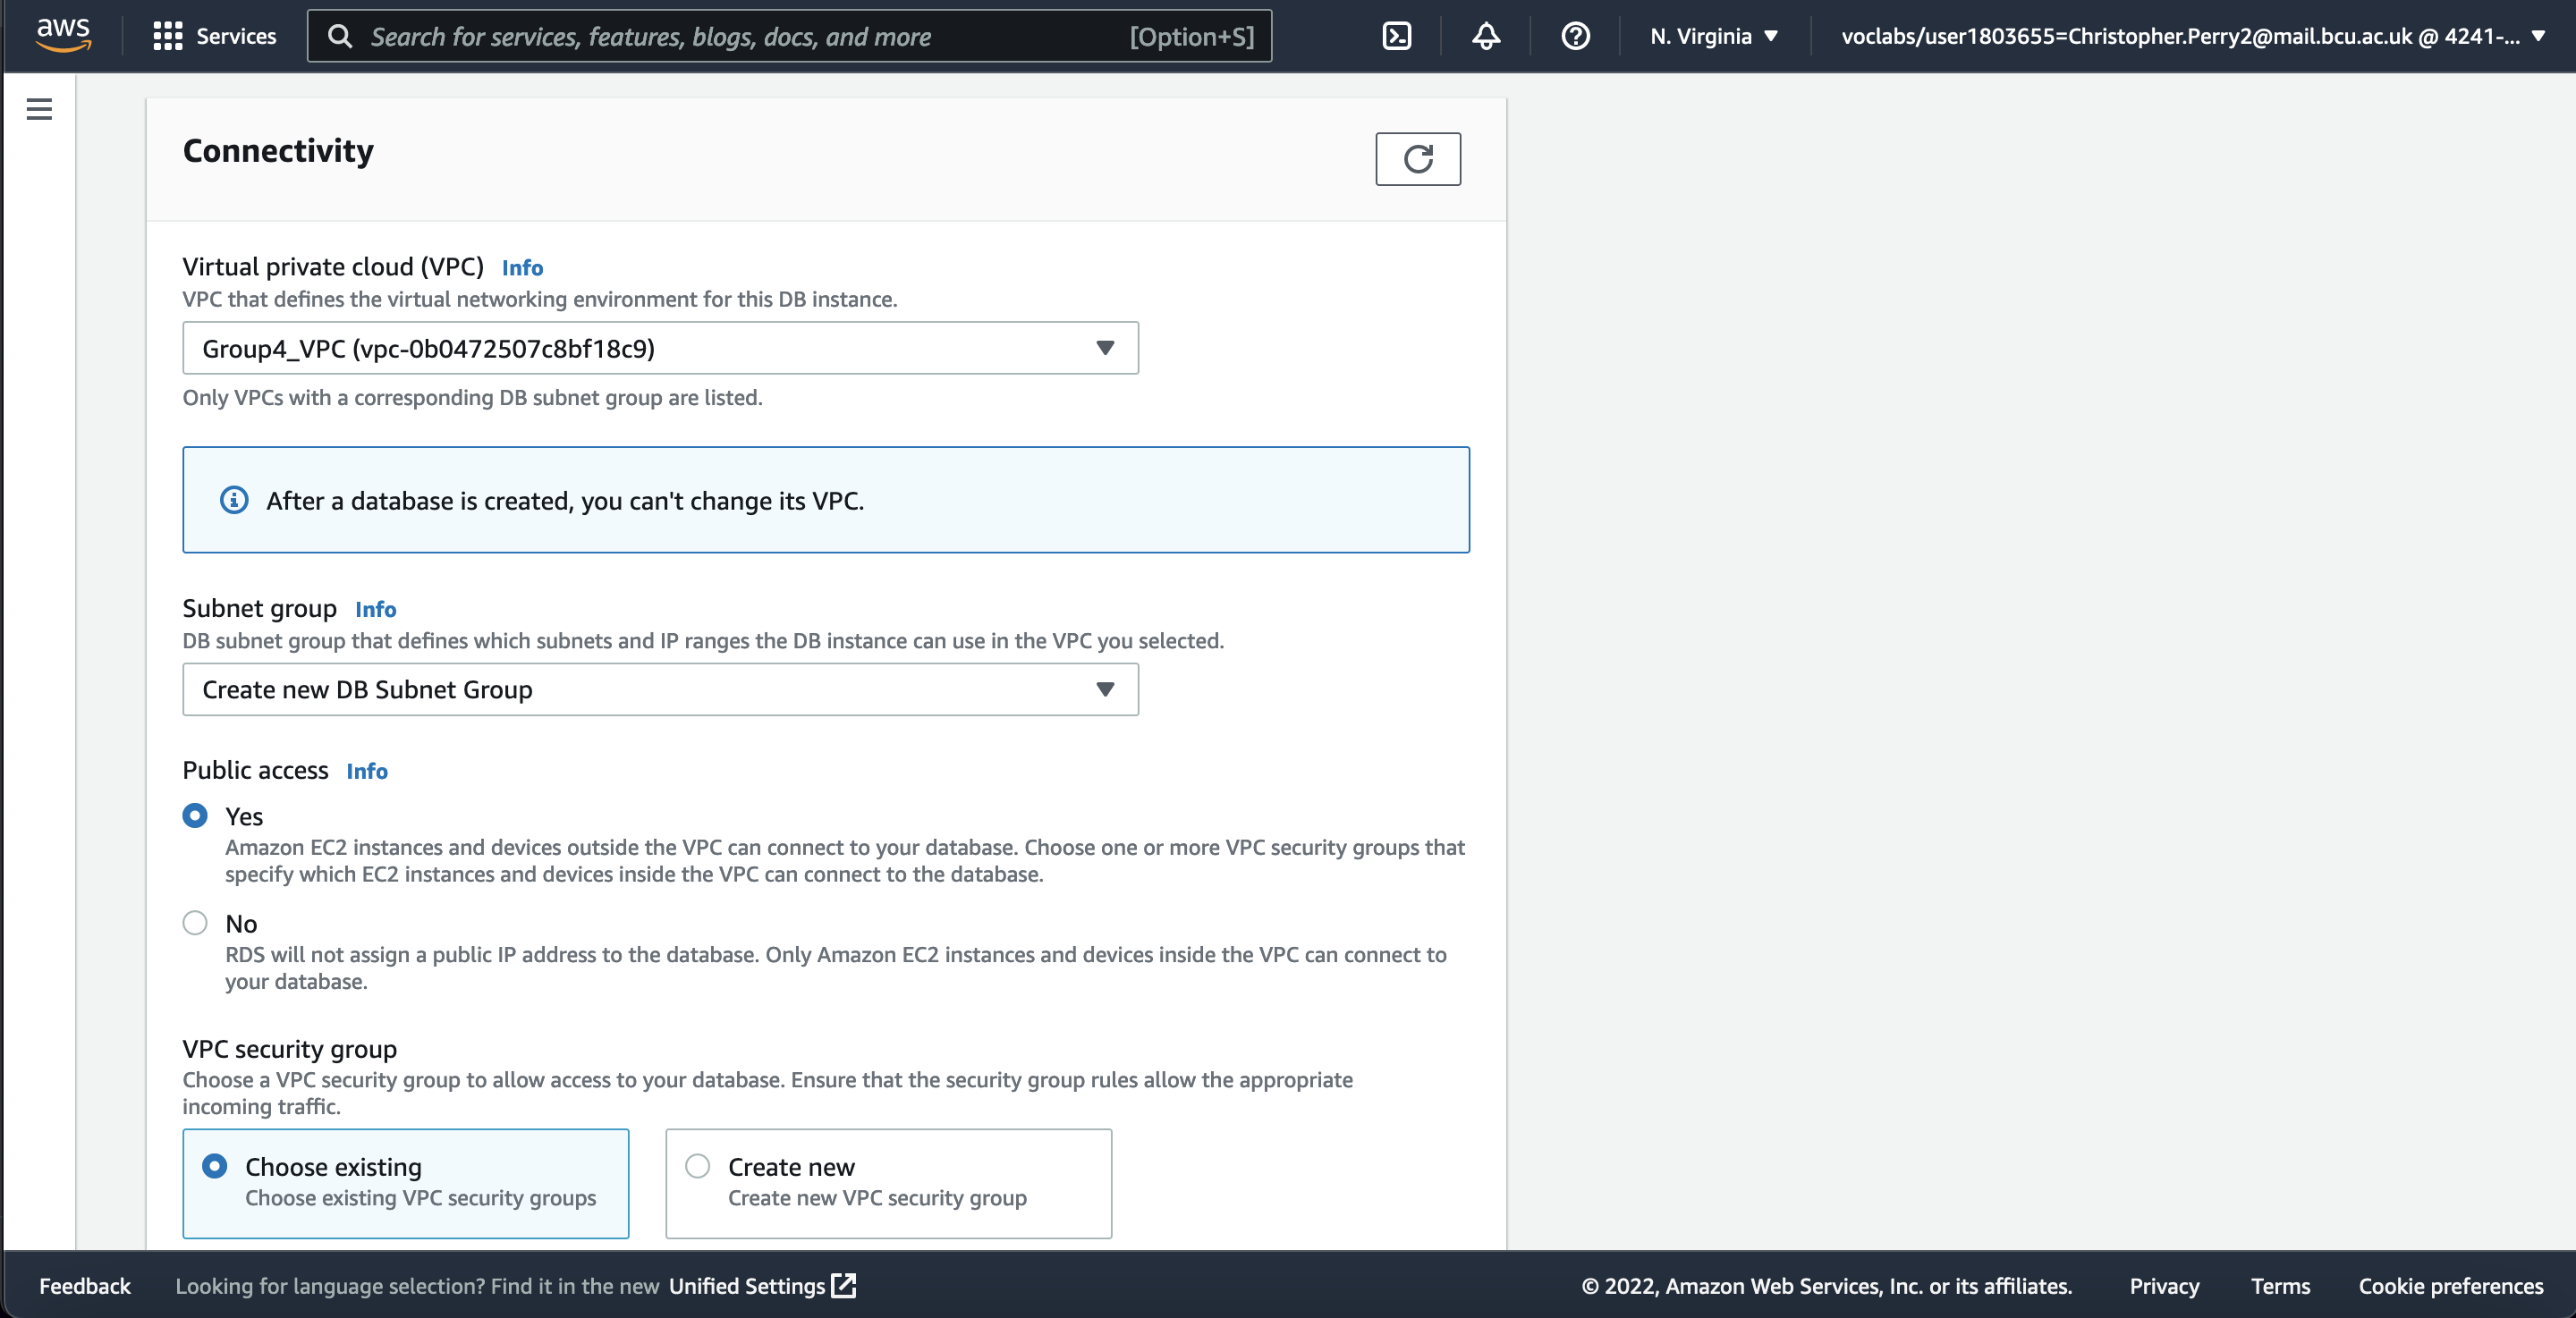
\includegraphics[width=\textwidth]{resources/rds/rds-connectivity-1}
    \caption{Selection of VPC and Subnet Groups.}
    \label{fig:rds-connect-2}
\end{figure}

Public access was turned off to further increase our application's security.

\begin{figure}
    \centering
    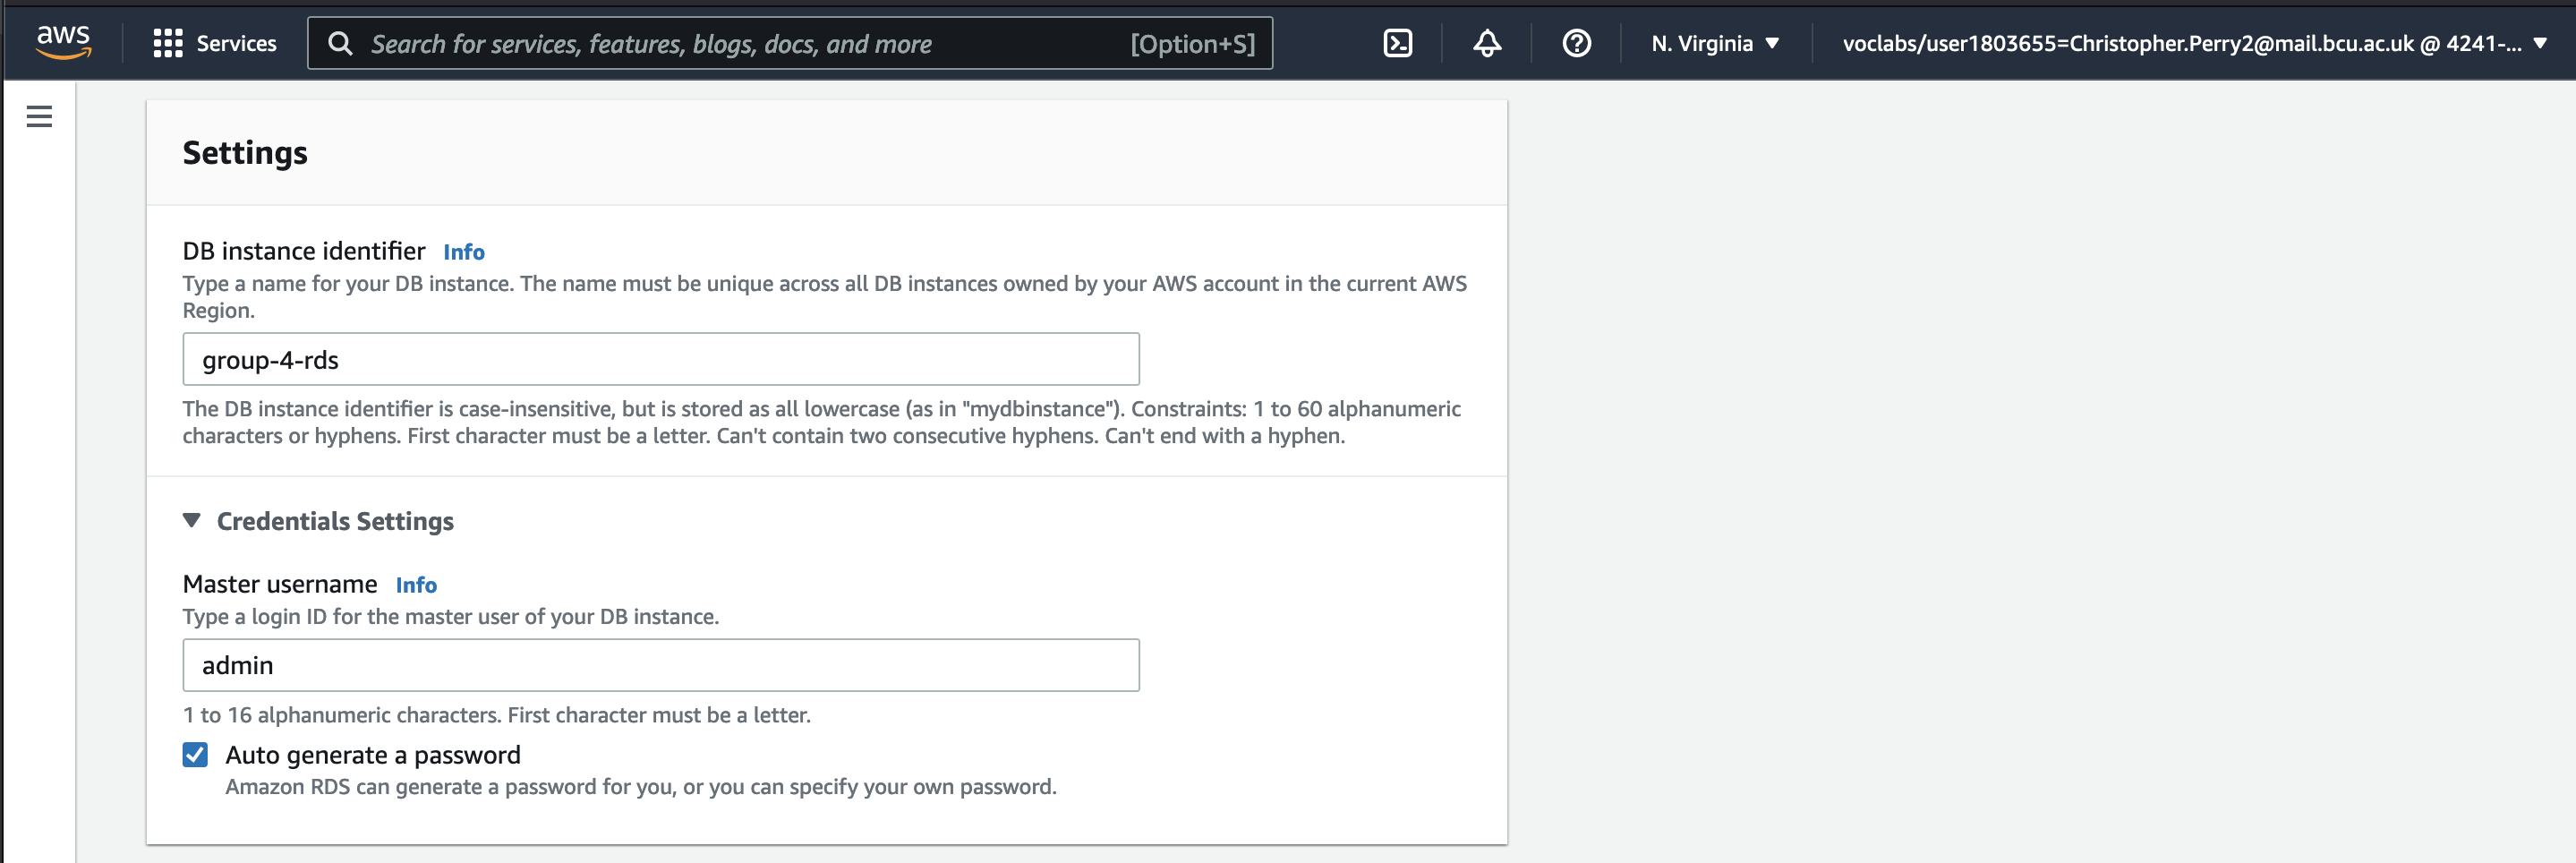
\includegraphics[width=\textwidth]{resources/rds/rds-settings}
    \caption{Credentials for RDS Authentication.}
    \label{fig:rds-settings-2}
\end{figure}

We selected an automatically generated password to ensure that it was created with current best security practices.